\documentclass{article}
\usepackage{comment,listings,framed,graphicx,url,xcolor}
\usepackage{amssymb}
\usepackage{amsthm}
\usepackage{mathtools}
\usepackage{graphicx}
\usepackage{amsmath}
\usepackage{mhchem}
\usepackage{physics}
\usepackage{hyperref}
\usepackage{fullpage}
\usepackage[margin=1in]{geometry}

\usepackage{soul}
\usepackage{listings}
\usepackage{color}

\usepackage{graphicx}
\usepackage{mathtools}

\usepackage[utf8]{inputenc}
\usepackage{booktabs}
\usepackage{siunitx}
\usepackage{graphicx}
\usepackage{pgfplots}

\usepackage{enumitem}
\usepackage{siunitx}
\usepackage{booktabs}
\usepackage{array}
\usepackage{makecell}
\usepackage{tabularx}

\usepackage{tikz}
\usetikzlibrary{positioning, arrows.meta, calc}

\usepackage[linguistics]{forest}

\definecolor{dkgreen}{rgb}{0,0.6,0}
\definecolor{gray}{rgb}{0.5,0.5,0.5}
\definecolor{mauve}{rgb}{0.58,0,0.82}
\definecolor{light}{rgb}{1,1,0.6}

\newenvironment{amatrix}[1]{%
  \left[\begin{array}{@{}*{#1}{c}|c@{}}
}{%
  \end{array}\right]
}

\lstset{
  language=Matlab,
  basicstyle=\ttfamily,
  keywordstyle=\color{blue},
  stringstyle=\color{purple},
  commentstyle=\color{green},
  morecomment=[l][\color{magenta}]{\#}
}

\usepackage{tikz}
\usetikzlibrary{positioning}

\usepackage{tabularray}
\newcommand\xx{$\displaystyle\frac{a+b}{a-b}=0$}
\newcommand\yy{$\displaystyle\int_a^bf(x)\,\textrm{d}x=\frac{a-b}{a+b}$}
\newcommand\zz{\fcolorbox{cyan3}{yellow9}{\parbox{\dimexpr\linewidth-2\fboxsep-2\fboxrule\relax}{\dummy}}}


\usepackage{chemfig}
\usepackage{mathrsfs} 
\usepackage{enumitem}

\newcommand{\mycomment}[1]{}

\title{Coalition Shuffling Formalism}
\author{Marley McWilliams}

\begin{document}

\maketitle
The foundation of the analysis is the modeling of a discrete, multiplayer, stochastic game as a finite directed acyclic graph, $\mathcal{G} = (V, E)$. This structure allows for a complete and deterministic solution to a system that includes both rational decision-making and chance.

\section{The State-Space Graph Formulation}

The game is entirely captured by its state-space graph, where vertices represent game states and edges represent state transitions.

\subsection{Vertices as Game States ($v \in V$)}
A vertex represents a complete, instantaneous snapshot of the game. Each state is formally defined by a tuple $(\mathbf{U}, p, C)$, where:
\begin{itemize}
    \item $\mathbf{U}$ is a vector of player utilities (e.g., health).
    \item $p$ is an integer identifying the active player whose turn it is to act.
    \item $C$ is the state of the primary chance-based element (e.g., the sequence of remaining rounds).
\end{itemize}

\subsection{Node Classification}
Vertices are partitioned into three types, governing how their value is calculated:
\begin{enumerate}
    \item \textbf{Terminal Nodes:} States where the game has concluded. Their value is a fixed utility vector representing the outcome (e.g., $[1, 0, 0]$ for a Player 1 victory).
    \item \textbf{Decision Nodes:} States where an active player $p$ must choose an action from a set of available moves. Each action corresponds to a directed edge to a successor state.
    \item \textbf{Chance Nodes:} States where the transition is determined by a probabilistic event (e.g., the initial permutation of the chance element $C$). Edges emanate to all possible outcomes, each weighted by its probability.
\end{enumerate}

\section{The Solution Concept: Generalized Expectiminimax}

To "solve" the graph is to compute an expected utility vector for every node, representing the win probabilities for each player assuming optimal play from that state forward. This is achieved via the \textbf{Expectiminimax algorithm}, applied recursively from the terminal nodes.

The value $E(v)$ of a node $v$ is a vector of expected utilities and is determined by its type:

\begin{itemize}
    \item If $v$ is a \textbf{Terminal Node}, $E(v)$ is its predefined outcome vector.

    \item If $v$ is a \textbf{Chance Node}, its value is the probability-weighted average of its successors' values. For all successors $v_i$ with transition probabilities $P(v_i)$:
    \begin{equation}
        E(v) = \sum_{i} P(v_i) \cdot E(v_i)
    \end{equation}

    \item If $v$ is a \textbf{Decision Node} for player $p$, the logic assumes rational agency. Player $p$ will choose the action leading to a successor state $v_i$ that maximizes their component of the expected utility vector, $E_p(v_i)$. Therefore:
    \begin{equation}
        E(v) = E(v_k) \quad \text{where} \quad k = \text{max}_{i} E_p(v_i)
    \end{equation}
\end{itemize}
This backward induction guarantees a definitive value for every state, predicated on the assumption that all players act optimally to maximize their own win probability.

\section{State-Space Reduction via Equivalence Classes}

A naive enumeration of the state space is combinatorially intractable. The model's feasibility relies on aggressive state-space reduction by identifying and merging equivalent nodes.

\begin{itemize}
    \item \textbf{Symmetric Equivalence:} States that are permutations of one another (e.g., player healths $(4, 2)$ for player 1 is symmetric to $(2, 4)$ for player 2) are normalized into a single canonical representation.

    \item \textbf{Behavioral Equivalence:} A more powerful concept where two distinct nodes are deemed equivalent if they are of the same type and their sets of outgoing edges lead to probabilistically identical distributions of successor equivalence classes. An iterative refinement algorithm identifies these classes, merging nodes that are functionally indistinguishable.
\end{itemize}

This process transforms the complete state-space graph into a minimal, canonical \textbf{quotient graph} that preserves all strategic information while being computationally tractable. This foundational analysis yields the fully annotated state-space map, where each node is a game state and each edge is labeled with the calculated expected utility vector. This solved graph serves as the empirical basis for subsequent investigations into path analysis, decision theory, and player dynamics.

\section{Deriving Model stuff}

Consider the state-space maps for $\boxed{142,1}\to\boxed{100}$ under expectiminimax (free-for-all) conditions:
\begin{figure}[h]
    \centering
    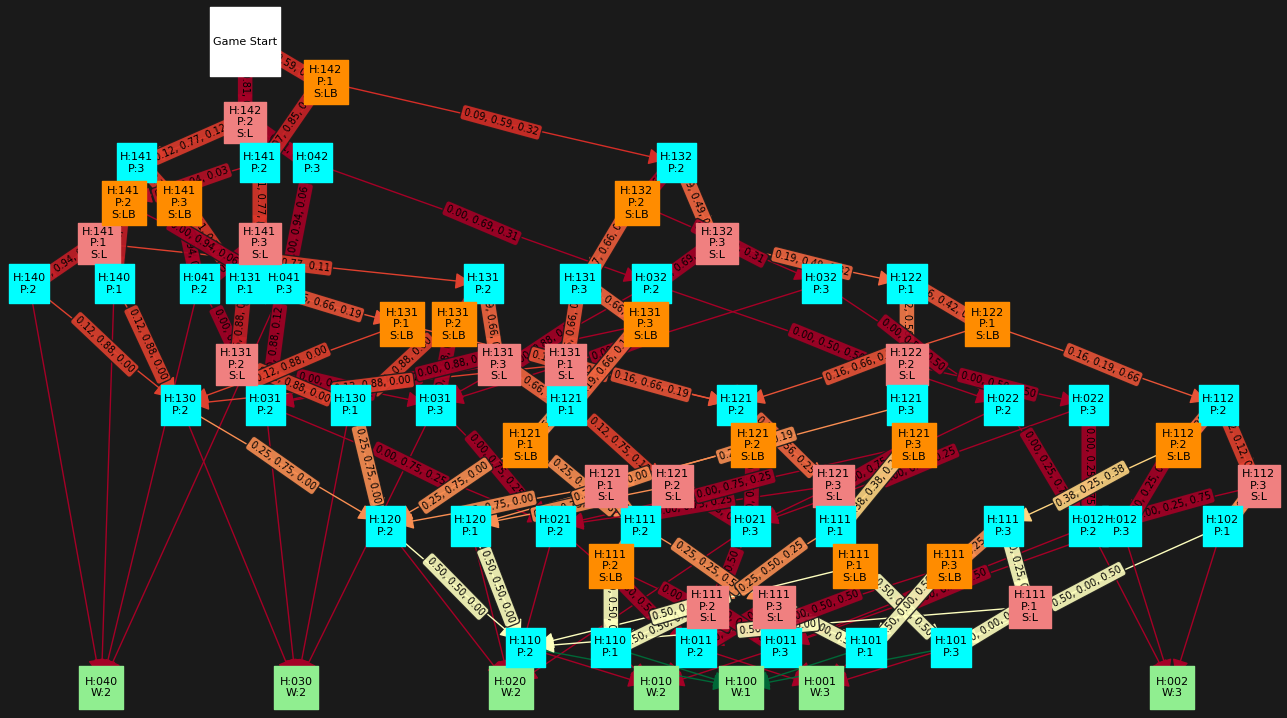
\includegraphics[width=0.9\linewidth]{142wL11.png}
\end{figure}
\\
One such path is given here:
\begin{align*}
    \boxed{142,1}&\to\boxed{142,2}\to\boxed{141,3}\to\boxed{141,1}\to\boxed{131,2}\to\boxed{131,3}\\
    &\to\boxed{121,1}\to\boxed{121,2}\to\boxed{120,1}\to\boxed{110,2}\to\boxed{100}
\end{align*}
The probability of each player's victory is given in descending order with probability-based events (currently uniform) denoted $P$ (attacks only with $1\to 2\equiv 1\text{ attacks }2$) and decisions $D$ linked to the posterior node. Due to decision pruning, which can be reversed, it does not account for failed action attempts.
\begin{equation}
    \boxed{100}\equiv\left[ \begin{array}{@{}*{11}{c}@{}}
        0.05&0&0.12&0.12&0.12&3/16&3/16&1/8&1/4&1/2&1\\
        0.7&0.81&0.77&0.77&0.77&21/32&21/32&3/4&3/4&1/2&0\\
        0.25&0.19&0.12&0.11&0.11&5/32&5/32&1/8&0&0&0\\
        &P&D&P&D&P&D&P&D&P&P\\
        &&2\to3&&1\to2&&3\to2&&1\to2&&
    \end{array} \right]\equiv\boxed{142,1}
\end{equation}
This path involved consistent bad luck for 2, 3 always attacking 2, 1 attacking 2 without recourse and 2 playing sub optimally in $\boxed{142,2}\to\boxed{042,3}$. Taking the difference between path scores:
\begin{equation}
    D_{\text{path}-\text{alt}}=\left[ \begin{array}{@{}*{11}{c}@{}}
        -0.09&+0.12&+0.12&+0.01&+0.13&+0.19&-0.13&+0.25&+0.50&+1.00\\
        +0.22&-0.04&+0.00&-0.17&-0.22&-0.22&+0.19&+0.00&-0.50&-1.00\\
        -0.13&+0.08&-0.01&+0.11&+0.09&+0.03&-0.06&-0.25&+0.00&+0.00\\
        P&D&P&D&P&D&P&D&P&P\\
        &2\to3&&1\to2&&3\to2&&2\to3&&
    \end{array} \right]
\end{equation}
This is distinguished from the difference between future and incident paths (provides "comfort level" with individual path prior to committing to calculating all paths).
\begin{equation}
    D_{\text{path}-\text{in}}=\left[ \begin{array}{@{}*{11}{c}@{}}
        -0.05&+0.12&+0.01&0&0.07&0&-1/16&+1/8&+1/4&+1/2\\
        +0.11&-0.04&0&0&-0.12&0&-3/32&0&-1/4&-1/2\\
        -0.06&-0.07&-0.01&0&0.05&0&-1/32&-1/8&0&0\\
        &P&D&P&D&P&D&P&D&P\\
        &&2\to3&&1\to2&&3\to2&&2\to3&
    \end{array} \right]
\end{equation}
This equips the user with a naive objective function, akin to assessing one perspective but not yet exhausting options (conversely, there are excitable theorists with little background knowledge). Notice $D_{\text{path}-\text{alt}}=D_{\text{path}-\text{in}}-D_{\text{alt}-\text{in}}$.
\\
\\
Let $X,Y\in\mathbb{R}^n$ where $D$ impacts other $D$'s differentially as filtered through $P$.
More generally, over some boundary which contains a collection of $D$: for incident paths $X$ and projective paths $Y$, we have $M=YX^T-XY^T=\left(D_iP_j-P_iD_j\right)\mathbf{e}_{ij}$ where the column space of $M$ represents. Letting $\chi,\gamma$ represent the "strategic potential" at any game point, denoted by the gradient of red-green as derived from expectiminimax, setting $v$ as the gradient of strategic gives $M_{c}=\left(\frac{\partial\chi_j}{\partial\gamma_i}-\frac{\partial\chi_i}{\partial\gamma_j}\right)\mathbf{e}_{ij}=\nabla\times v$, implying that "tension" between strategies comes explicitly from vorticity between paths. Notice $v$ conforms perfectly to expectinimimax when perturbations are not present, so players act rationally according to incentives. However, when a player is at a disadvantage, they can make use of $M_c$ to gauge and shift the momentum of the game according to strategic objectives. This is why real-world, irrational social dynamics are complex: irrational perturbations are continuously introduced to static frameworks, producing dynamic behavior. As nodes elevate and consideration paths elongate, this turns into coordinating strategies.
\\
\\
Given the decision spread $D$, we want the vector orthogonal to the space spanned by the perturbations of each vector from a reference (typically average, can include special instructions/information/formatting). The space spanned by those differences represent a subspace for exploration and cross-domain connection. When normalized, we have the following least squares solution:
\begin{align*}
    d_{\text{avg}}&=\frac{1}{\left|D\right|}\sum_{d\in D}d\tag{$d_{\text{ref}}$ often this}\\
    W_{\text{Dis}}&=\text{span}\left\{\forall d\in D: d-d_{\text{ref}}\right\}\\
    &=\text{QR}\left(\sum_{d\in D}\left(d-d_{\text{ref}}\right)\mathbf{e}_d\right)\tag{Column space}\\
    W_{\text{Dis}}^\perp&=\text{null}\left(\sum_{d\in D}\left(d-d_{\text{ref}}\right)\mathbf{e}_d^\perp\right)
\end{align*}
As more paths are calculated, more similarities and differences can be categorized.
\\
\\
There exists a $D_{[\alpha,n]}=D_{\text{out}-\text{alt}}$ at node $\alpha$ with depth $n$ corresponding with each path of length $l\leq n$, where horizontal size corresponds with $n$:
\begin{align*}
    \text{INT}&=\lim_{n\to\infty}D_{[0,n]},\tag{0 nodes are axioms}\\
    \text{ where }D_{[\alpha,k]}&\to\left[D_{[\alpha+1,k-1]},D_{[\alpha+2,k-2]},\cdots,D_{[\alpha+i,k-i]},\cdots,D_{[k-1,\alpha+1]},D_{[k,\alpha]}\right]
\end{align*}
As such it creates a linear system of "desired decisions" (those which end at $\boxed{100}$ here) in accordance with other player decisions at certain nodes. I haven't done the math yet, but everyone simulates both the game and everyone else's simulation of the game. Some decisions will be more circumstantial to individual players, meaning they're willing to invest more strategic loss in order to posture. And that posturing will need some type of credibility calculation, which I'll work on.
\\
\\
Uh, this implies posture is dynamically related. D can be found by building up, which helps parameterize the dynamics. We can also build structures iteratively. $S$ can be intentionally adjusted via institutions. The trick is to maximize the utility of $D_Y$ in order to learn. Next, let's assume $S$ and $D$ are non-constant and behave dynamically.
\\
\\
Even if this could convert statics to dynamics, how can we gauge the phase space at play? Because relationships between individuals will be some matter of alignment and misalignment on issues, it's akin to polarity across molecules. Individuals maneuvering through crowds tend to act like fluid particles, it's possible this connection has more to do with the interaction of rational actors than anything unique to the human mind. In that case, our objective becomes to design an enzyme which produces certain "static" protein structures from some inputs. The enzyme itself operates by controlling stabilizing and guiding the differential system we're describing, which corresponds with competent designs we can build to formalize incentive networks.
\newpage
Let's simulate a simpler game fully:
\begin{figure}
    \centering
    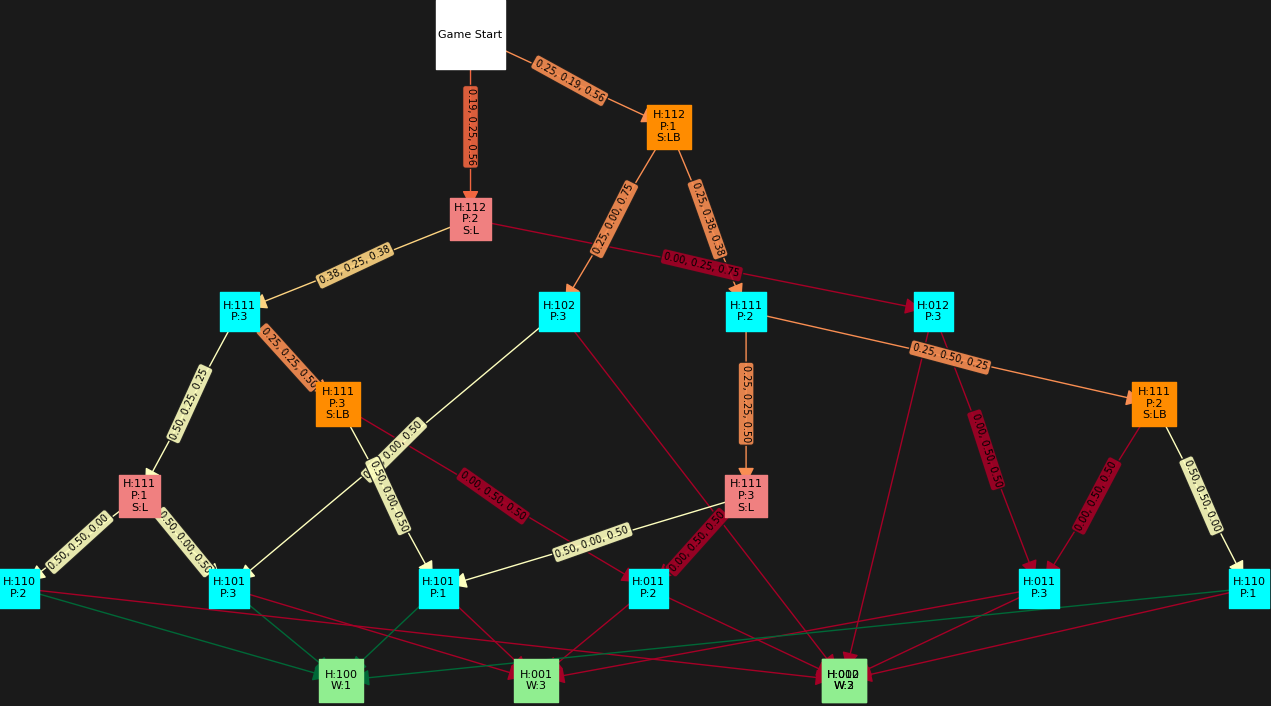
\includegraphics[width=0.5\linewidth]{112wL11.png}
    \caption{Enter Caption}
    \label{fig:placeholder}
\end{figure}
\newpage
A new configuration should allow for non-zero sum games and aim for outcomes with mutually beneficial results. But what on earth should this look like?
\end{document}

